\title{background}
\begin{center}
    \textbf{Chapter 02}\\
   \section{ \large \textbf{Literature Review}}
\end{center}
\subsection{Introduction}
In the dynamic world of business, organizations of all sizes rely heavily on their workforce to achieve success. Effectively managing employees is crucial for optimizing productivity, fostering a positive work environment, and ensuring overall business growth. To achieve these goals, modern businesses have turned to technology, giving rise to employee management systems. An employee management system is a comprehensive software solution designed to streamline and automate various Human Resources (HR) processes within an organization. It serves as a centralized platform where HR professionals and managers can efficiently handle essential employee-related tasks, such as maintaining personnel records, tracking attendance, managing performance evaluations, handling payroll, and facilitating communication between employees and management.
\subsection{Overview}
An employee management system is a comprehensive software solution designed to
facilitate and streamline various Human Resources (HR) processes within an organization.
It serves as a central platform where HR professionals and managers can efficiently manage
and organize employee-related tasks, data, and interactions. The primary goal of an
employee management system is to optimize HR operations, enhance employee engagement,
and ultimately contribute to the overall success of the organization. The evolution of
employee management systems can be traced back to the 1980s when businesses started
transitioning from manual, paper-based HR processes to computerized systems. Early
versions of HR software focused on basic tasks like employee data storage, attendance
tracking, and payroll management, bringing greater accuracy and efficiency to these
processes.
\newpage
\subsection{Platform Choice}
When choosing a platform for an employee management system, organizations have several
options to consider based on their specific needs, budget, and technical requirements. The
choice of platform can significantly impact the system's performance, accessibility, security,
and scalability. Here are some common platform choices for employee management systems:
Cloud-based Platform: Cloud-based employee management systems are hosted on remote
servers and accessed via the internet. This platform offers several advantages, including:
Accessibility: Users can access the system from anywhere with an internet connection,
promoting remote work and mobile access.
Scalability: Cloud platforms can easily scale resources to accommodate the growing needs of
an organization without significant hardware investments.
Cost-effectiveness: Organizations can avoid upfront hardware and infrastructure costs, as
cloud providers usually charge based on usage or a subscription model.
Data Backup and Security: Cloud providers often implement robust data backup and security
measures to safeguard sensitive employee information.
\subsection{Software Choice}
When considering software choices for an employee management system,
organizations have a wide array of options to meet their specific needs. The software
selected will significantly impact how efficiently and effectively HR processes are
managed within the organization. Here are some popular software choices for an
employee management system. Dedicated HR management software is designed
specifically to handle various HR functions comprehensively. These systems typically
include features for employee records, attendance tracking, performance management,
payroll processing, benefits administration, and more. They offer a centralized solution
to streamline HR operations and improve overall efficiency. HRIS platforms focus on
managing and organizing HR-related data. They typically include modules for employee
information, attendance, leave management, reporting, and analytics. HRIS software is
suitable for organizations looking for a system tailored specifically to their HR needs.
Some organizations opt for integrated ERP software that includes HR modules as part of
a larger suite. ERP systems offer a unified platform for various business functions like
finance, supply chain, and HR. Integration with other departments can enhance data flow
and facilitate seamless information sharing.
\newpage
\subsection{Development Methodology}
The development of an employee management system typically follows a structured software
development methodology to ensure efficiency, quality, and successful project completion.
Several methodologies are commonly used in software development, and the choice of
methodology depends on the project's scope, timeline, team size, and complexity. Here are
some popular development methodologies applicable to employee management system
projects. The Waterfall methodology is a traditional and linear approach to software
development. It follows a sequential process where each phase must be completed before
moving to the next. The phases typically include requirements gathering, design,
implementation, testing, deployment, and maintenance. This method is suitable for well-
defined projects with stable requirements deployment process. Ultimately the development
methodology used by employee management system will depend on their specific needs and
goals. By carefully considering the available options and selecting the methodology that best
fits their business model, they can ensure that their e-commerce platform is developed
efficiently and effectively.
\vspace{4.5mm}
\begin{figure}[h]
    \centering
    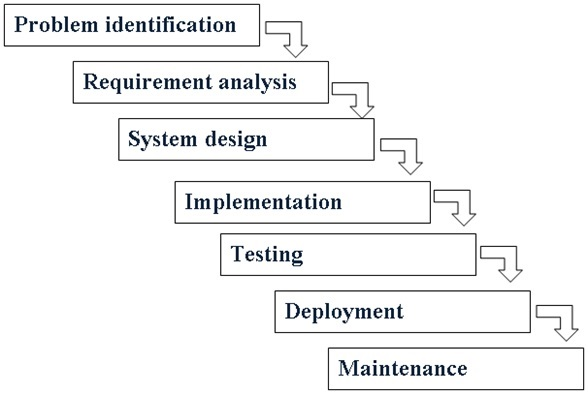
\includegraphics[height=8cm]{img/waterfall-method.jpg}
    \caption{Waterfall Model}
    \label{fig:waterfallmodel}
\end{figure}
\newpage
\subsection{Conclusion}
The evolution of employee management systems has transformed the way organizations
manage their workforce and HR processes. From their humble beginnings as computer-
based tools in the 1980s to the sophisticated cloud-based solutions of today, employee
management systems have become essential assets for businesses of all sizes. The central
role of these systems is to streamline and automate HR tasks, creating a more efficient and
productive work environment. By maintaining comprehensive employee profiles, tracking
attendance and leave, managing performance evaluations, handling payroll, and fostering
communication, employee management systems optimize HR operations and improve
overall workforce management. Cloud-based platforms have brought remarkable
advantages, such as increased accessibility, scalability, and cost-effectiveness. Cloud
solutions have empowered businesses to embrace remote work and ensure real-time data
access from anywhere, contributing to a more flexible and agile workforce. Furthermore, the
software choice for an employee management system plays a pivotal role in its success.
Whether it's dedicated HR management software, integrated ERP solutions, cloud-based
Saabs platforms, or open-source options, organizations must carefully select the software
that aligns with their specific needs and long-term goals. Moreover, the development
methodology employed in creating these systems is crucial. Whether following the linear
approach of Waterfall, the iterative nature of Agile, or a combination of both in Spiral
methodology, choosing the right development methodology ensures efficient project
completion, high-quality deliverables, and adaptability to changing requirements.